\section[Clustering]{Piecewise Emulation via Clustering \& Classification}

\providecommand{\bbeta}{\boldsymbol{\beta}}
\providecommand{\bgamma}{\boldsymbol{\gamma}}
\providecommand{\Sglobal}{S_{\mathrm{global}}}

\begin{frame}{Standard Surrogates Near Discontinuities}
    \begin{columns}[c]
        \begin{column}{0.5\textwidth}
            \begin{itemize}
                \item Standard GPs and PCEs assume global smoothness.
                \item Spectral methods suffer from the Gibbs phenomenon (oscillations near the jump).
                \item GPs smear boundaries \& artificially inflate uncertainty everywhere.
                \item Result: A surrogate model we cannot fully trust for virtual certification.
            \end{itemize}
        \end{column}
        \begin{column}{0.5\textwidth}
            \centering
            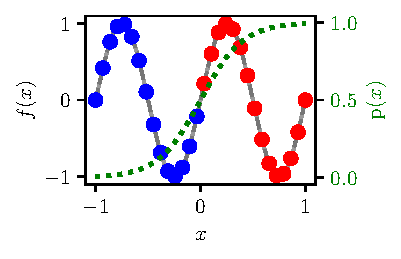
\includegraphics[width=0.9\textwidth,height=0.4\textheight,keepaspectratio]{../figures/sota_2/gp_realizations_demo.pdf}
        \end{column}
    \end{columns}
\end{frame}

\begin{frame}{The Need for a Problem-Independent Approach}
    \begin{itemize}
        \item Complex simulations (e.g., in-flight icing) feature abrupt regime transitions without explicit flags.
        \item Prior expert knowledge to manually partition the input space ($\bx$) is rarely available.
        \item We need a \textbf{data-driven learning} strategy to discover discontinuities automatically.
        \item Goal: Cluster data, train local models, and define boundaries with \textbf{no manual hand-holding}.
    \end{itemize}
\end{frame}

\begin{frame}{Proposed Methodology: Iterative Coupling}
    \begin{block}{Piecewise Surrogate Model Formulation}
        We can think of our surrogate as a patchwork of simpler, local models glued together by a classifier:
        \begin{equation}
            \tilde{f}(\bx; \bbeta, \mathcal{P}) = \sum_{l=1}^L \mathbb{I}_{\Omega_l}(\bx; \bgamma) \tilde{f}_l(\bx; \bbeta_l)
        \end{equation}
    \end{block}
    \vspace{0.2cm}
    \begin{itemize}
        \item $\bz$: Tells us which data points belong to which cluster.
        \item $\mathbb{I}_{\Omega_l}(\bx; \bgamma)$: The classifier that draws the boundaries between regions.
        \item $\tilde{f}_l(\bx; \bbeta_l)$: Our localized experts (the regressors).
        \item \textbf{The hard part:} We have to jointly optimize the memberships, boundaries, and model parameters without getting trapped in bad local minima.
    \end{itemize}
\end{frame}

\begin{frame}{The Algorithmic Loop}
    \centering
    \vspace{0.3cm}
    \begin{tikzpicture}[
        node distance=1cm and 1.5cm,
        block/.style={rectangle, draw=black, fill=blue!10, text width=2.8cm, text centered, rounded corners, minimum height=1.2cm, thick},
        arrow/.style={-{Stealth[scale=1.2]}, thick}
    ]
        % Nodes
        \node[block] (clust) {1. Propose New\\ $\bz^{(t+1)}$};
        
        \node[block, right=of clust] (regress) {2. Update Local\\ $\bbeta^{(t+1)}$};
        \draw[arrow] (clust) -- (regress);
        
        \node[block, below=of regress] (class) {3. Update Classifier\\ $\bgamma^{(t+1)}$};
        \draw[arrow] (regress) -- (class);
        
        \node[block, left=of class] (score) {4. Evaluate Global\\ Score $\Sglobal$};
        \draw[arrow] (class) -- (score);
        \draw[arrow] (score) -- (clust);
    \end{tikzpicture}
    
    \vspace{0.5cm}
    \begin{itemize}
        \item Instead of solving everything at once, we use an iterative approach.
        \item We start with a rough guess and let the local models dictate how to improve the clusters.
        \item Because the loop is modular, you can plug in whatever regressor or classifier you prefer.
    \end{itemize}
\end{frame}

\begin{frame}{Model-Based Clustering \& Global Score}
    \begin{block}{Global Score Function $\Sglobal$}
        We measure how good our patchwork model is by summing up the local scores (like log-marginal likelihoods):
        \begin{equation}
            \Sglobal(\bbeta, \bz) = \sum_{l=1}^L S(\bbeta_l, \data_l(\bz))
        \end{equation}
    \end{block}
    
    \begin{itemize}
        \item By keeping the score local, we can actually train all our regressors in parallel.
        \item We decide whether to move a point to a new cluster by checking if it improves this overall score ($\Delta S$).
        \item But there's a catch: if we just greedily maximize the score, the algorithm might create tiny, meaningless clusters just to fit the noise perfectly.
    \end{itemize}
\end{frame}

\begin{frame}{Stochastic Membership Updates \& Convergence}
    To stop the model from overfitting, we introduce some randomness controlled by a "temperature" parameter:
    
    \begin{equation}
        \mathbb{P}(l \rightarrow l^{\prime}) \propto \exp \left( \frac{1}{T} \Delta S \right) \, h\left(\mathbb{P}_{\mathrm{CLS}}(l^\prime \mid \bx, \bgamma) \right)
    \end{equation}

    \begin{itemize}
        \item \textbf{Exploration (High $T$):} When things are "hot", the classifier's uncertainty drives the bus. Points can freely jump across boundaries to explore new setups.
        \item \textbf{Exploitation ($T \rightarrow 0$):} As we cool things down, the model becomes greedy, locking into the best score.
    \end{itemize}
    
    \begin{block}{Convergence Properties}
        From a mathematical standpoint, this cooling process guarantees that we eventually settle on a stable, optimal partition (or enter a mild, easily detectable limit cycle).
    \end{block}
\end{frame}

\begin{frame}{The Evolution of Model-Based Clustering}
    \begin{center}
        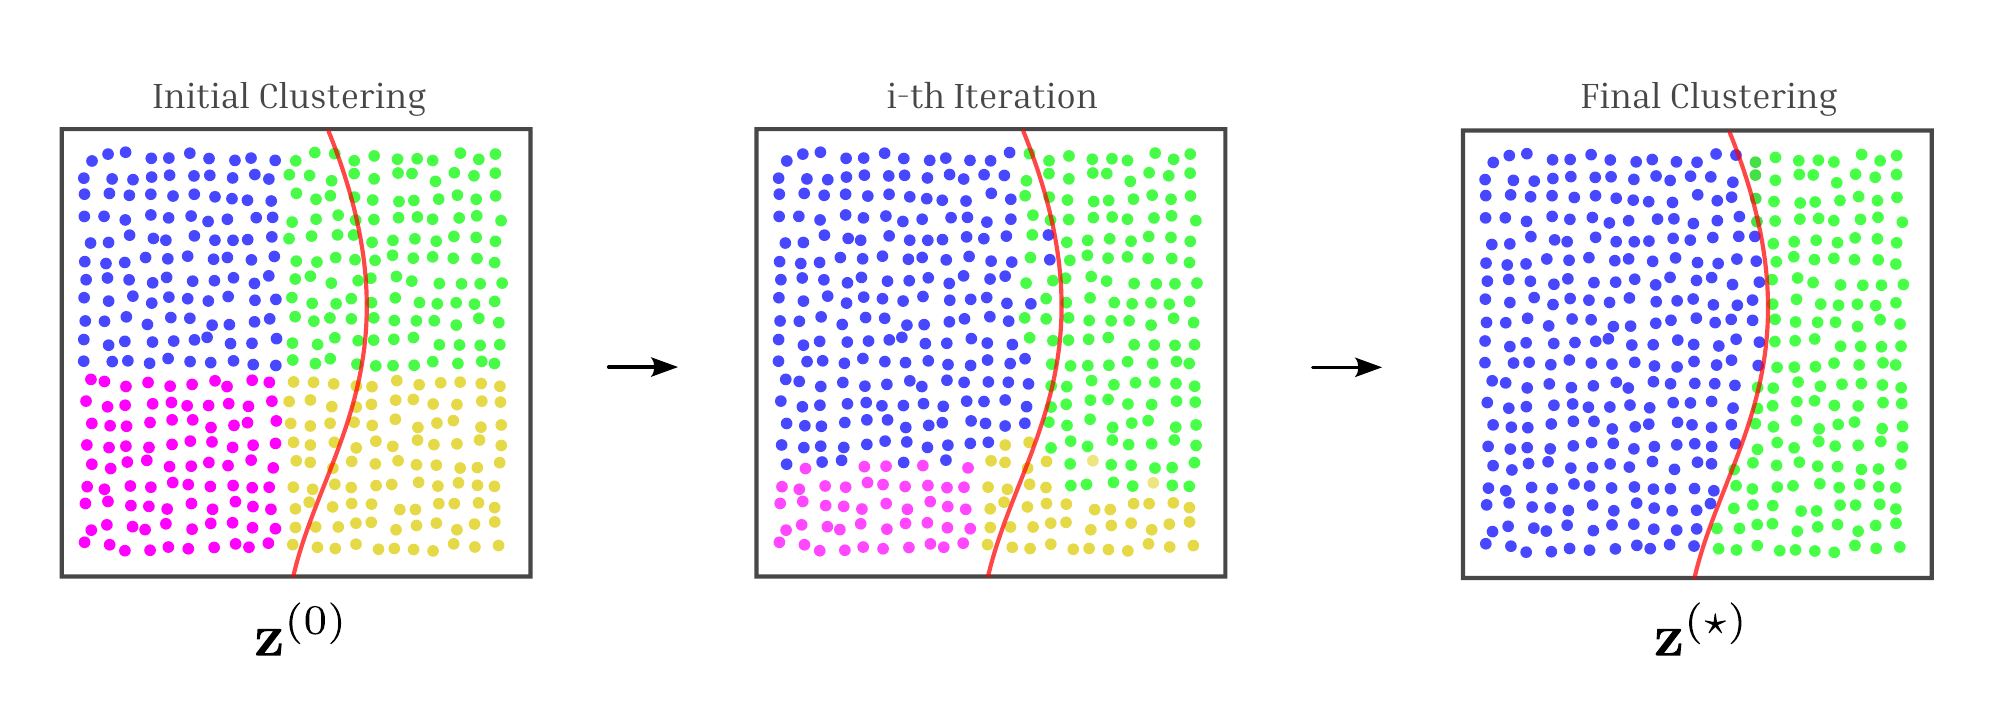
\includegraphics[width=0.85\textwidth,height=0.6\textheight,keepaspectratio]{../figures/clustering/Evolution.png}
    \end{center}
    \vspace{0.2cm}
    \begin{itemize}
        \item The algorithm iteratively discovers both the boundaries (classifier) and the smooth physical regimes (regressors) simultaneously.
    \end{itemize}
\end{frame}

\begin{frame}{Numerical Example 1: 1D Jump}
    \begin{columns}[c]
        \begin{column}{0.4\textwidth}
            \begin{itemize}
                \item Let's look at a simple 1D function with a sharp jump.
                \item A naive clustering (e.g., K-Means or single GP) gets it completely wrong by trying to smooth across the jump.
                \item The proposed algorithm neatly pinpoints the exact location of the jump, recovering a \textbf{good clustering} without Gibbs oscillations.
            \end{itemize}
        \end{column}
        \begin{column}{0.6\textwidth}
            \centering
            Naive approach:\\
            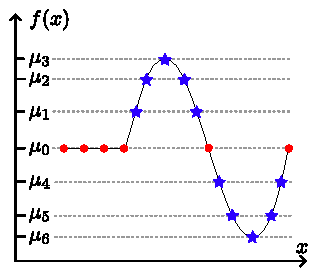
\includegraphics[width=0.8\textwidth,height=0.35\textheight,keepaspectratio]{../figures/clustering/badClustering.pdf}\\
            Our approach:\\
            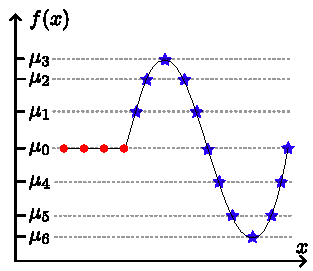
\includegraphics[width=0.8\textwidth,height=0.35\textheight,keepaspectratio]{../figures/clustering/goodClustering.pdf}
        \end{column}
    \end{columns}
\end{frame}

\begin{frame}{Numerical Example 2: Higher Dimensions}
    \begin{columns}[c]
        \begin{column}{0.5\textwidth}
            \begin{itemize}
                \item In higher dimensions, the boundaries between physical regimes can take on complex, non-convex shapes.
                \item Thanks to the stochastic annealing, the algorithm doesn't easily get trapped in bad local configurations.
                \item By pairing it with a strong classifier, we can trace out highly irregular boundaries effortlessly.
                \item It neatly separates the data without us ever having to label the physics manually.
            \end{itemize}
        \end{column}
        \begin{column}{0.5\textwidth}
            \centering
            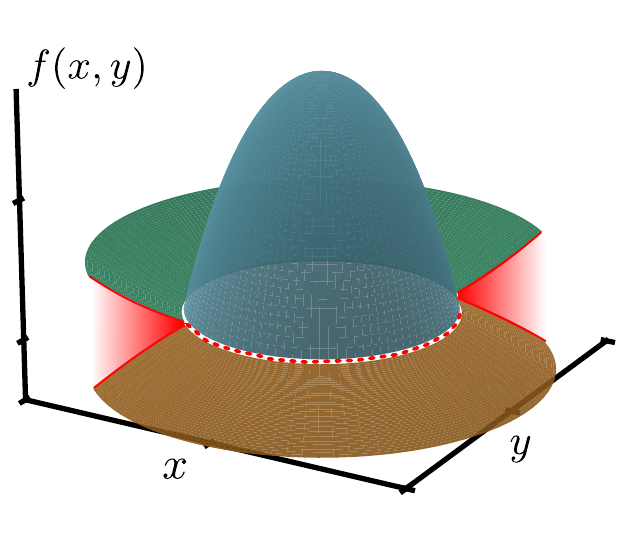
\includegraphics[width=0.9\textwidth,height=0.35\textheight,keepaspectratio]{../figures/clustering/function_plot_compressed.png}\\
            \vspace{0.2cm}
            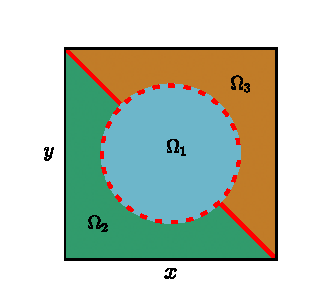
\includegraphics[width=0.9\textwidth,height=0.35\textheight,keepaspectratio]{../figures/clustering/partition_plot.pdf}
        \end{column}
    \end{columns}
\end{frame}

\begin{frame}{Taming Over-Clustering}
    \begin{columns}[c]
        \begin{column}{0.5\textwidth}
            \begin{itemize}
                \item \textbf{Risk:} Over-segmenting perfectly smooth domains.
                \item \textbf{Solution:} Merge adjacent clusters using a classifier "confusion metric".
                \item \textbf{Result:} A highly robust, hands-off workflow for handling tricky physics.
            \end{itemize}
        \end{column}
        \begin{column}{0.5\textwidth}
            \centering
            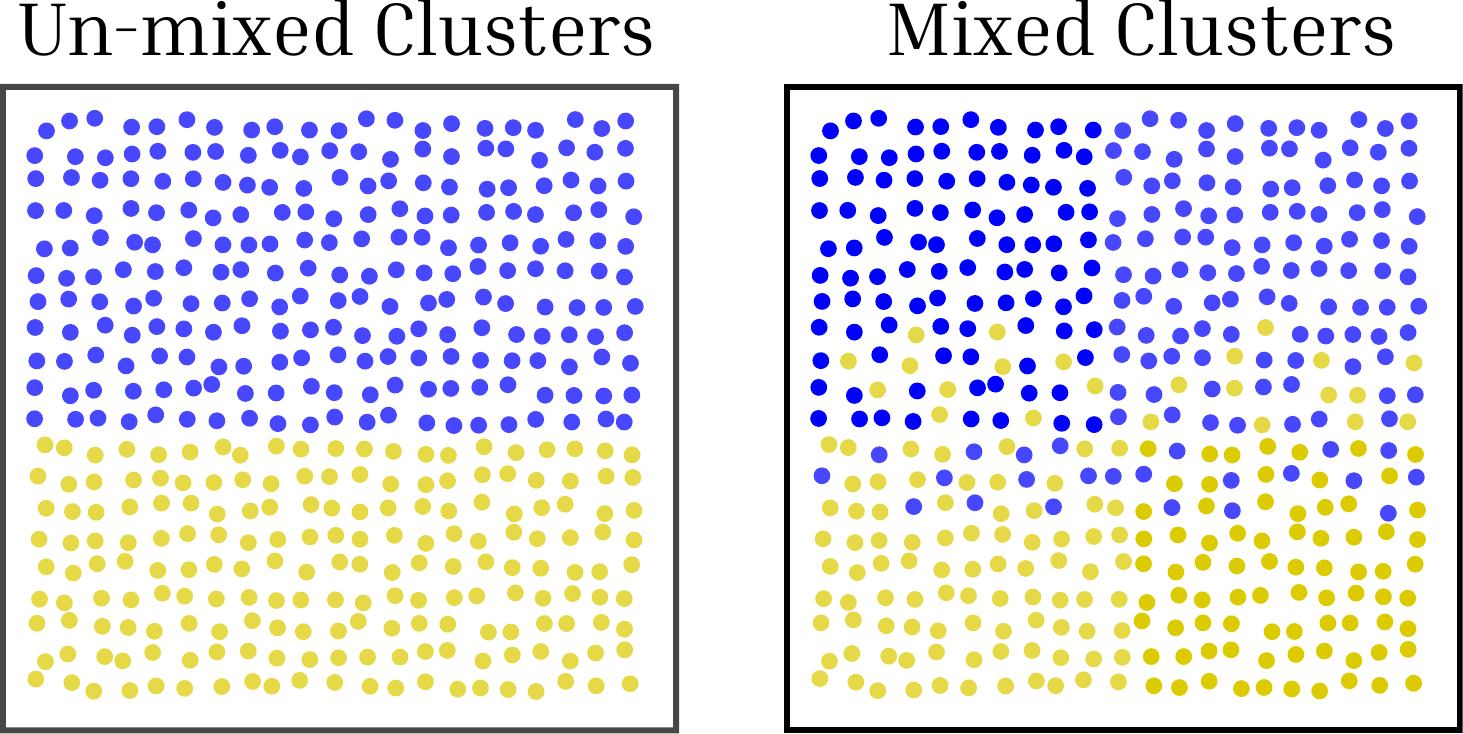
\includegraphics[width=0.9\textwidth]{../figures/clustering/confusion.png}
        \end{column}
    \end{columns}
\end{frame}
